\documentclass[10pt,twocolumn,letterpaper]{article}
\usepackage[T1]{fontenc}
\usepackage[review]{cvpr}
\usepackage{graphicx,amsmath,amssymb,booktabs,microtype,multirow}
\definecolor{cvprblue}{HTML}{176D89}
\definecolor{oursteal}{HTML}{008C88}
\usepackage[pagebackref,breaklinks,colorlinks,allcolors=cvprblue]{hyperref}
\def\confName{CVPR}\def\confYear{2027}
\newcommand{\R}{\mathbb{R}}
\title{Beyond Visual Agreement:\\Compositional Mechanics for Position-Driven Deformable Twins}
\author{Anonymous submission}
\setlength{\textfloatsep}{9pt plus 1pt minus 1pt}
\setlength{\dbltextfloatsep}{9pt plus 1pt minus 1pt}
\setlength{\floatsep}{7pt plus 1pt minus 1pt}
\setlength{\intextsep}{7pt plus 1pt minus 1pt}
\begin{document}
\twocolumn[{
\renewcommand{\twocolumn}[1][]{#1}
\maketitle
\begin{center}
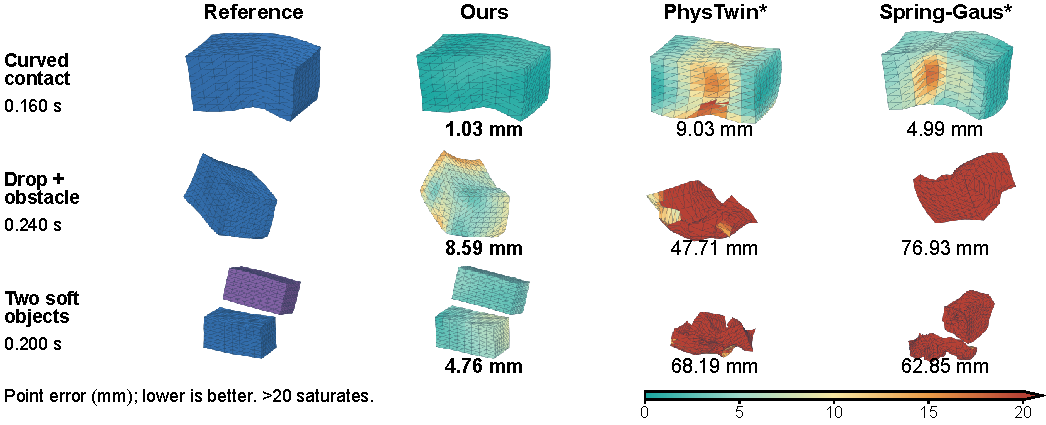
\includegraphics[width=.98\textwidth]{figures/cohesive-teaser.pdf}
\par\vspace{2pt}
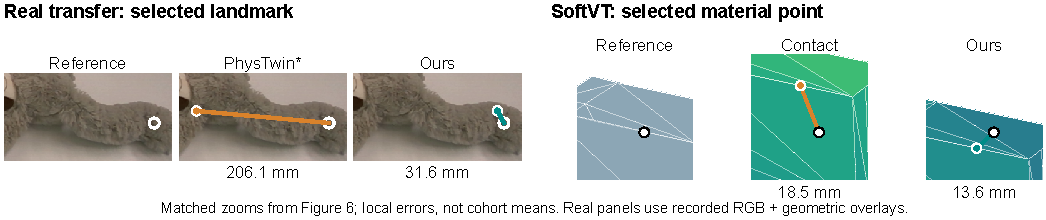
\includegraphics[width=.98\textwidth]{figures/public-wins-teaser.pdf}
\captionof{figure}{\textbf{Changed interactions: simulation and public-dataset successes.} Top: saved final-frame forecasts for curved contact, obstacle drop and two soft bodies (first world/query); shared cameras, scales and point-error colors. Labels give frame RMS; * denotes baseline adaptations. Bottom: matched zooms from Fig.~\ref{fig:publicwins}, with local 3D errors. Real panels overlay predictions on recorded RGB. These selected examples complement the full-cohort results.}
\label{fig:teaser}
\end{center}
}]
\begin{abstract}
A deformable reconstruction can match observed images without identifying the physical response to a new interaction. We study position-driven twins that separate material-attached constitutive response, tool-relative attachments, world-space interactions and Gaussian appearance. Compact energy decoders are pretrained and frozen; scene parameters are fitted to observed positions, then queried with new tool trajectories or initial conditions. We instantiate this representation in controlled coupled mechanics, a reduced manipulation adapter and a real-object equilibrium adapter, with their different assumptions explicit. Across six simulated interaction families and 24 material worlds, motion RMS is 1.97\,mm versus 10.80 and 11.27\,mm for adapted PhysTwin and Spring-Gaus, while a matched analytic control achieves 1.84\,mm. Slip-aware prediction reduces average error across 40 fresh SoftVTBench episodes, and a two-pair real-transfer pilot improves tracking from 44.63 to 39.16\,mm over a frozen PhysTwin adaptation. The full real continuation benchmark still favors PhysTwin. An exact scale ambiguity and an additional-observation experiment explain why rendering, physical response and uncertainty must be evaluated separately. Visual agreement alone does not identify physics.
\end{abstract}

\section{Introduction}
A soft toy held between two grippers may deform because its material is compliant, its attachment is loose, or both. Different explanations can reproduce a visible shape yet respond differently when a gripper moves or releases. A camera orbit helps reveal geometry, but cannot measure a force that leaves that geometry unchanged. For a useful digital twin, the key test is what happens after the interaction changes.

Gaussian scene models coupled to mechanics already support reconstruction, simulation and novel interactions~\cite{xie2024physgaussian,zhong2024springgaus,jiang2025phystwin}. Learned constitutive models provide reusable material knowledge~\cite{ma2023nclaw,mittal2025uniphy}. We build on these advances with a concrete composition: bulk response belongs to material coordinates; compliant attachments relate material to tools; gravity and collision geometry belong to the world; appearance follows the predicted state. Tool positions are inputs and reaction forces follow from mechanics. This organization permits an interaction to change without redefining the fitted material.

Our question is whether this composition improves prediction beyond the fitted motion, and how to measure that improvement. We distinguish three forms of evidence. Controlled simulations expose the underlying state and test new loads, supports and contacts. A prospective manipulation study tests placement and release on a public simulated dataset. Real captures test ordinary continuation and a small, geometry-qualified transfer to another interaction. Their adapters share physical roles, not one universal solver or checkpoint.

Physical accuracy is not a single visual score. We report world motion, internal deformation and, when reference physics permits, momentum/contact diagnostics. A shared appearance model measures the image consequences of the predicted motion. An exact scaling example shows that identical images can accompany different reactions. A separate inverse experiment shows that one more position observation can improve held-out motion and force prediction, even while uncertainty becomes overconfident.

Our contributions are: (1) a position-driven composition of compact bulk and attachment energies with explicit environmental terms and Gaussian transport; (2) an observability-based account of what geometry can and cannot identify; and (3) a multi-protocol evaluation of changed interactions, physical diagnostics and rendered agreement, retaining strong analytic and simple-motion controls. The strongest gains occur in controlled interaction transfer; real continuation and posterior calibration expose remaining limitations.

\begin{figure*}[t]
\centering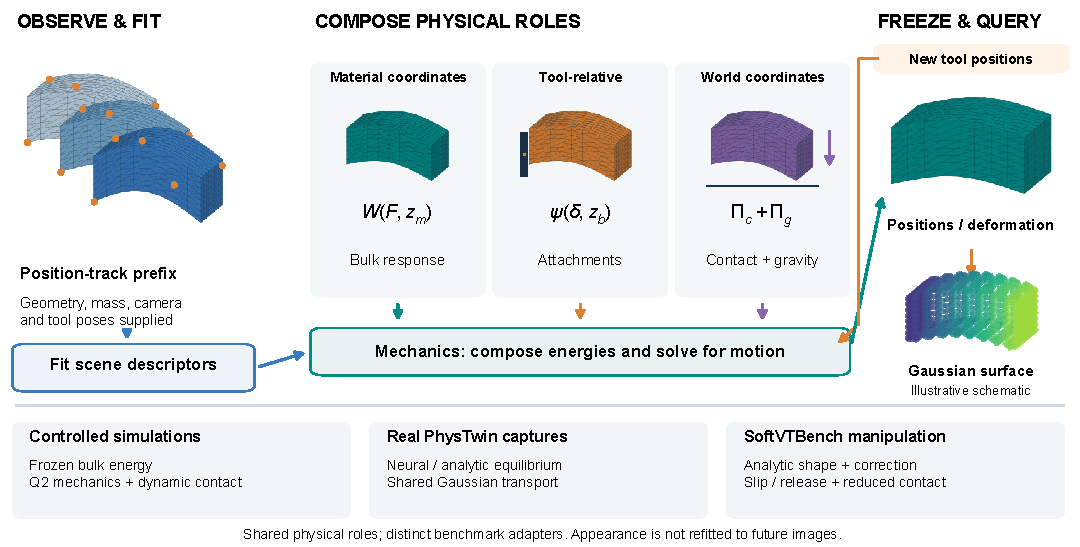
\includegraphics[width=\textwidth]{figures/cohesive-method.pdf}
\caption{\textbf{Fit physical roles, freeze the scene, query a new interaction.} Material descriptors move with the object, attachment targets follow tools, and loads/contact act in the world. Geometry and correspondences are supplied. The controlled simulator uses coupled Q2 mechanics; real PhysTwin uses tetrahedral equilibrium; SoftVT uses an analytic shape anchor with a reduced pose/contact rollout. These are explicit instantiations of the representation, not the same checkpoint. Gaussian appearance is evaluated separately.}
\label{fig:method}
\end{figure*}

\section{Related Work}
\paragraph{Physical visual representations.}
3D Gaussian splatting provides explicit spatial appearance~\cite{kerbl2023gaussians}. PAC-NeRF combines radiance fields with differentiable continuum simulation for system identification~\cite{li2023pacnerf}. PhysGaussian transports Gaussian primitives through continuum deformation with supplied material and boundary conditions~\cite{xie2024physgaussian}. Spring-Gaus learns spring-mass dynamics and appearance from multi-view video~\cite{zhong2024springgaus}. PhysTwin uses sparse RGB-D interaction videos, geometry priors and lifted tracks to fit spring-mass physics and Gaussian appearance; it already demonstrates future motion and novel interactions~\cite{jiang2025phystwin}. We do not claim priority for simulatable reconstruction or physics--appearance separation. Our study isolates changed-interaction response and the distinct sources of its error.

\paragraph{Reusable mechanics and inverse identification.}
NCLaw learns constitutive laws within known equations and studies transfer across geometry and boundary conditions~\cite{ma2023nclaw}. UniPhy pretrains latent-conditioned constitutive networks and freezes them while adapting a scene latent~\cite{mittal2025uniphy}. Our scalar energy follows this established reuse principle, derives stresses by differentiation, and composes bulk response with separately parameterized interfaces. DiffPD addresses efficient differentiable mechanics and contact~\cite{du2022diffpd}; i-PhysGaussian and Boba address integration robustness and efficient twin simulation~\cite{cao2026iphysgaussian,pang2026boba}. We compare configured physical pipelines rather than attributing every difference to the constitutive network.

\paragraph{Plausibility, reconstruction and evaluation.}
PhysDreamer and OmniPhysGS use generative priors to produce plausible physical dynamics~\cite{zhang2024physdreamer,lin2025omniphysgs}. PIDG combines time-dependent Gaussian deformation, velocity and stress with momentum residuals and optical-flow supervision~\cite{hong2026pidg}. These objectives differ from forecasting a reset system under new controls; our supplementary PIDG comparison tests dense appearance reconstruction with a learned mechanics constraint, separately from changed-action prediction. SoftVTBench supplies simulated visuotactile manipulation episodes~\cite{jing2026softvt}; PhysTwin and Deform360 supply real deformable-object captures~\cite{jiang2025phystwin,li2026deform360}. We use SoftVT and PhysTwin under explicitly defined position-input protocols, not their native end-to-end leaderboards.

\section{Compositional Position-Driven Mechanics}
\subsection{State and physical roles}
Let $X\in\Omega_0$ denote a material point, $x(X,t)$ its world position and $F=\partial x/\partial X$ its deformation gradient. Initial geometry and correspondences are supplied. Observations contain positions $y_t$ and validity masks $V_t$ over a prefix; tools provide known poses. A query supplies subsequent tool motion, environmental geometry and, for dynamics, initial state and gravity. No future object positions or measured force trajectory are needed.

The scene potential separates four terms:
\begin{align}\label{eq:total}
\Pi(x;z,a)={}&\int_{\Omega_0} W_\theta(F;z_m(X))\,dV\nonumber\\
 &+\sum_b\int_{\Gamma_b}w_b(X)\psi_b(x-T_b(a);z_b)\,dA\nonumber\\
 &+\Pi_{\mathrm{contact}}(x;z_e)-\int_{\Omega_0}\rho g^\top x\,dV.
\end{align}
Here $z_m$ is material-attached, $T_b$ is a tool-relative target, and $z_e$ defines environmental geometry/contact. A Gaussian or tapered footprint $w_b$ localizes an attachment and is normalized over reference area. The primary controlled/real adapters use $\psi_b(\delta)=K_b\|\delta\|^2/2$. A bilateral attachment is different from unilateral collision contact: it can pull as well as push. The present models specify these roles rather than discovering arbitrary contact graphs from RGB.

\subsection{Shared energy and scene descriptors}
Define $C=F^\top F$, $J=\det F>0$, $I_1=\mathrm{tr}C$ and $I_2=((\mathrm{tr}C)^2-\mathrm{tr}(C^2))/2$. Our frozen energy uses invariant coordinates
\begin{equation}
q_1=J^{-2/3}I_1-3,\quad q_2=J^{-4/3}I_2-3,\quad v=J-\log J-1,
\end{equation}
and a positive-coefficient expansion
\begin{equation}\label{eq:bulk}
W_\theta(F;s,h,f)=e^s E_0\sum_{j=1}^{7}a_{\theta,j}(h,f)b_j(F),
\end{equation}
with $E_0=12000$\,Pa and $b=[q_1/2,q_2/2,v,q_1^2,q_1^3,\phi_1(q_1),\phi_2(q_1)]$ and $\phi_i(q)=\mathrm{softplus}(\alpha_iq)-\log2-\alpha_iq/2$. A $2\!\to\!16\!\to\!7$ SiLU decoder with softplus outputs supplies $a_j>0$; the decoder and positive slopes contain 169 parameters. Stress is $P=\partial W/\partial F$. Invariants enforce objectivity and isotropy, but do not prove global stability or universal material coverage.

We pretrain on 4,096 synthetic strain coupons spanning 18 compressible Mooney--Rivlin/Yeoh-type descriptor combinations, using 6,000 Adam steps, batch size 256, normalized stress MSE and a 0.1-weighted energy term. We freeze these weights before scene adaptation. Spatial scale descriptors and, where enabled, an independent positive volumetric multiplier are then fitted from the observed prefix. The controlled six-family study fixes $(h,f)=(0,-1)$ and fits a common smooth spatial scale family, including an offset for a second body. The real adapter fits a six-kernel material field and global nonlinear descriptors. The analytic controls replace the bulk energy with a known constitutive family.

Compliant attachment energy can be represented by a separate conditional positive-basis decoder, with quadratic springs as a special case. In the unknown-descriptor inverse experiment, stiffness, nonlinearity and Gaussian footprint centers/widths are fitted. In the six-family benchmark, fixture compliance and collision geometry are supplied; its results therefore test unknown material under known boundaries, not boundary recovery. Real attachments use tool-conditioned quadratic penalties. The supplement specifies each active parameter set.

\subsection{Fitting, dynamics and reduced adapters}
For fixed correspondences $A$, observable positions are $\hat y_t=y_0+A(x_t-X)$. Scene adaptation solves
\begin{equation}\label{eq:fit}
\min_z\sum_{t\in\mathcal T_o}\|V_t\odot(\hat y_t(z)-y_t)\|^2+\lambda\mathcal R(z),
\end{equation}
with shared weights frozen. Equilibrium solves $R=\nabla_x\Pi=0$ by damped Newton; implicit sensitivities satisfy
\begin{equation}
H\,\partial_z x=-\partial_z R,\qquad H=\partial_xR.
\end{equation}
The controlled dynamic study instead fits bounded descriptors by derivative-free prefix-loss optimization and integrates $M\ddot x=-\nabla_x\Pi$. Parameters are sealed before changed queries. Best finite prefix candidates are retained when optimization budgets expire; finite forecast coverage does not imply converged identification.

\paragraph{Controlled coupled mechanics.}
Q2 hexahedra, consistent mass and velocity Verlet model deformable bodies, compliant fixtures and conservative normal penalty contact. A translating finite-mass sphere receives equal-and-opposite contact forces. The evaluated coupled scenes do not include general rigid rotation, friction or continuous collision detection. Geometry, density and boundary recipes are known.

\paragraph{Real geometry and equilibrium.}
PhysTwin's reconstructed initial cloud supplies filtered tetrahedra and interpolation to tracked points. The first configuration is an effective rest shape, so unknown prestress may bias fitted parameters. A 240-node adapter fits 18 prefix frames and predicts successive equilibria at future tool positions. Source material remains frozen when transferring to a different interaction. This quasistatic approximation is not the coupled dynamic solver above.

\paragraph{Manipulation, slip and release.}
SoftVT uses an analytic mechanics anchor with prefix-fitted pose/residual corrections. A Kabsch alignment separates rigid discrepancy from nonrigid residual; this is an explicit geometric decomposition, not an inferred rigid/soft object label. During grasp, the last eight shared prefix observations estimate centroid velocity relative to the gripper. Only its nonnegative gravity-direction component is retained. A fixed overlap budget of half the initial extent triggers release. After release, a rigid pose integrator applies gravity and static-scene impulses with Coulomb friction, zero restitution and penetration correction. These impulses do not feed back into elastic shape. Thus this adapter tests placement and release, not coupled impact deformation.

\subsection{Appearance and physical observables}
A separate Gaussian appearance asset follows the mechanical state. Continuum deformation-gradient transport maps canonical center/covariance by
\begin{equation}
\mu_t=x(q,t)+F(q,t)r,\qquad\Sigma_t=F(q,t)\Sigma_0F(q,t)^\top.
\end{equation}
The controlled six-family comparison instead applies the same declared transport to every method; real captures use a common 16-neighbor local rigid blend. Appearance is fixed within these physical-response comparisons, without future-frame refitting. A separate PIDG study jointly fits dense appearance and a soft mechanics constraint (supplement). These controls measure motion-induced image error, not native end-to-end radiance reconstruction quality.

\section{Observability and Physical Accuracy}
\paragraph{An exact scale ambiguity.}
In position-controlled equilibrium with no independent body load, multiply every stiffness-bearing term, including compliant contact, by $c>0$. Then $\Pi_c=c\Pi$: corresponding equilibria and rendered images are unchanged, while reactions $\partial\Pi/\partial a$ scale by $c$. This holds for corresponding branches even if equilibrium is not unique. Our numerical example doubles stiffness, obtains residual $4.85\!\times\!10^{-13}$\,N and byte-identical images from three cameras, while doubling reactions. The idealized symmetry excludes an unscaled numerical regularizer. More views cannot remove this particular ambiguity. Known gravity, known-mass timed dynamics or measured reactions can break it; geometry alone does not establish absolute stiffness.

\paragraph{Observations as experiments.}
A new camera can expose hidden deformation. A new action can excite a material or attachment mode absent from the original observations. In a six-object inverse experiment with known density, geometry and categorical families, we fit 15 continuous material/attachment descriptors from noisy positions. One added stretch observation reduces held-command coordinate RMSE from 0.3395 to 0.0802\,mm and unobserved reaction RMSE from 0.0961 to 0.0292\,N. The variance-guided policy chooses the same stretch on every object and ties the fixed policy. Nominal 90\% position coverage falls from 97\% to 33\%: better point predictions do not establish calibrated uncertainty or intelligent action selection.

\paragraph{A measurement hierarchy.}
We distinguish (i) held-response accuracy: world position, rigid-aligned shape and available reaction/impulse targets; (ii) numerical sanity: finite trajectories, residuals, orientation, contact gaps and reference refinement; and (iii) visual agreement: PSNR, SSIM, LPIPS and silhouette IoU under stated rendering controls. No weighted ``physical realism'' score collapses these different quantities. On real captures, positions and images are available, but force accuracy cannot be certified without additional measurements.


\begin{figure*}[t]
\centering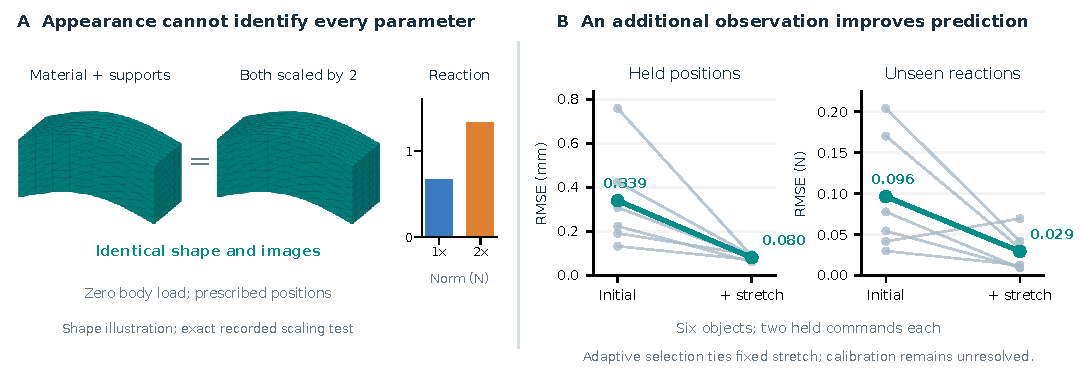
\includegraphics[width=\textwidth]{figures/cohesive-observability.pdf}
\caption{\textbf{What another observation can resolve.} Left: in a controlled load-free scale example, co-scaling stiffness preserves rendered geometry while doubling reaction; shapes are a schematic of this exact invariance. Right: a different six-object experiment with known gravity/density adds one stretch observation and improves held-command position and reaction predictions. Lines are individual objects. Adaptive selection ties this fixed action; calibration does not improve.}
\label{fig:observability}
\end{figure*}

\section{Experiments}
\subsection{Physical-response protocols}
Table~\ref{tab:protocol} states the input contract. We retain complete declared cohorts and report metrics in their native definitions: simulation uses point-vector RMS; SoftVT uses mean frame coordinate RMSE; real captures use mean pointwise Euclidean distance. We never pool these scores. Tests reuse known interaction families or named assets; ``changed interaction'' is more precise here than unrestricted OOD generalization.
\begin{table}[t]
\centering\small\setlength{\tabcolsep}{3pt}
\caption{\textbf{Evaluation contracts.} Geometry/correspondences are supplied throughout. All forecast parameters are fixed before their query.}
\label{tab:protocol}
\begin{tabular}{p{.22\columnwidth}p{.32\columnwidth}p{.32\columnwidth}}\toprule
Study & Observed / known & Held query\\\midrule
Six-family simulation & Prefix tracks; density, boundaries & 24 worlds, 48 changed interactions\\
SoftVTBench & 48 prefix tracks; tools, static scene & 40 fresh episodes; recurring assets\\
Real PhysTwin & Reconstructed tracks; tool positions & 8 continuations; 2 qualified transfer pairs\\\bottomrule
\end{tabular}
\end{table}

\subsection{Controlled changes in supports and contact}
Six scene families cover moving/released clamps, curved-obstacle pushing, container/obstacle drops, finite-mass rigid impact, two deformable bodies, and heterogeneous material. Four independently sampled material worlds per family each provide one calibration prefix and two changed queries. Queries vary fixture location, displacement, velocity, drop height/orientation or contact configuration. Object geometry and density are fixed in this study. Tracks sample a two-face material subset every 2\,ms; unknown material is fitted while boundary recipes are given.


\begin{figure}[t]
\centering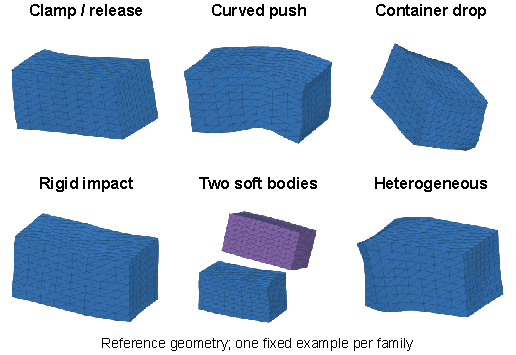
\includegraphics[width=\columnwidth]{figures/cohesive-families.pdf}
\caption{\textbf{Six physical query families.} Reference geometries from the fixed first world/query. Fixtures, contact geometry and density are supplied; material is inferred from a different calibration interaction.}
\label{fig:families}
\end{figure}

\paragraph{Comparators and fairness.}
We adapt the authors' PhysTwin and Spring-Gaus internal force/integration implementations to common geometry, observations and boundary interfaces. Both fit edge stiffness; their optimization parameterization and budgets differ from continuum fitting. PhysTwin damping is fixed to zero in this conservative benchmark. A Neo-Hookean analytic control knows the reference family but fits its parameters using the same continuum schedule. UniPhy's adapter supports only eight drop queries: one completes, seven encounter native CFL failures, and 40 are unsupported. We do not rank it from incomplete coverage or attribute adapter failures to the original method generally.

\begin{table}[t]
\centering\small\setlength{\tabcolsep}{3pt}
\caption{\textbf{Six-family interaction transfer, 48/48 forecasts for each row.} Motion and aligned shape: vector RMS (mm). Impulse error: N\,s. PSNR: common frozen appearance, noninitial frames. Bold denotes the best column value, including the analytic control.}
\label{tab:sim}
\begin{tabular}{lrrrr}\toprule
Method & Motion$\downarrow$ & Shape$\downarrow$ & Impulse$\downarrow$ & PSNR$\uparrow$\\\midrule
PhysTwin adapt. &10.80&5.94&.0500&25.68\\
Spring-Gaus adapt. &11.27&6.00&.0572&25.88\\
Ours &1.97&1.25&.0098&35.61\\
Analytic control &\textbf{1.84}&\textbf{1.16}&\textbf{.0086}&\textbf{36.02}\\\bottomrule
\end{tabular}
\end{table}

Ours reduces mean motion error relative to both native adaptations in every family. Across 24 worlds, paired differences are $-8.83$\,mm versus PhysTwin (world-bootstrap 95\% interval $[-12.18,-5.83]$) and $-9.30$\,mm versus Spring-Gaus ($[-12.40,-6.50]$). The difference from analytic is $+0.13$\,mm ($[-0.01,0.27]$): learned mechanics does not outperform the known reference family. The common appearance comparison favors the more accurate trajectories, but does not establish superior appearance reconstruction.


\begin{figure*}[t]
\centering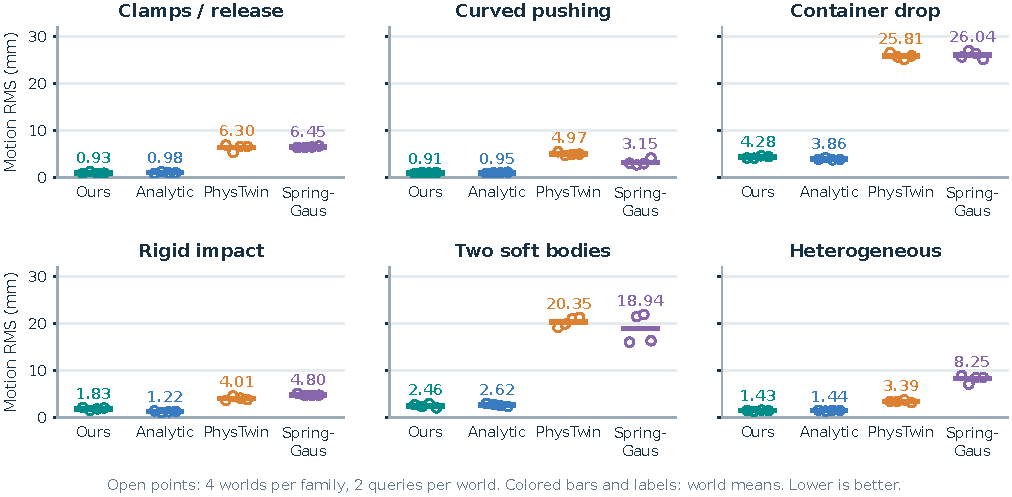
\includegraphics[width=\textwidth]{figures/cohesive-family-results.pdf}
\caption{\textbf{Every material world, separated by interaction family.} Each open point averages two changed queries of one world; bars and labels show four-world means. All four methods complete all 48 queries. Axes share the same range, and no frame-level confidence interval is implied. Ours improves both adapted spring models in every family; the matched analytic control remains competitive.}
\label{fig:familyresults}
\end{figure*}

\paragraph{Physical checks and reference sensitivity.}
Common sampled material-grid inversions occur in 0/48 queries for ours and analytic, 33/48 for PhysTwin and 37/48 for Spring-Gaus. Ours has no extra/missed contact events among 44 sampled event identities; the native adaptations have four/two extras, respectively. These are discrete diagnostics, not continuous nonintersection proofs. Eleven of twelve $n=4$ versus $n=6$ reference comparisons complete; one stacking run times out. Differences range from 0.027 to 0.931\,mm. On five fully paired refined worlds, our motion advantage remains 7.20\,mm over PhysTwin and 7.87\,mm over Spring-Gaus. This supports the ordering on that subset, not population-wide convergence. Full per-family, contact and rendering results are in the supplement.

\subsection{SoftVT: prospective manipulation forecasts}
Two released soft-object suites and two reserved tasks per suite provide ten fresh episodes per combination. The first 60\% supplies 48 selected upper-surface tracks at 20\,Hz; future robot commands and initial volumetric geometry are known. These are 40 new episodes of recurring assets, not unseen objects or an RGB/tactile policy leaderboard.
\begin{table}[t]
\centering\small
\caption{\textbf{SoftVT, all 40 fresh episodes and 1,998 frames.} Coordinate RMSE in mm. The slip update changes placement, not internal shape.}
\label{tab:soft}
\begin{tabular}{lr}\toprule
Method & Error$\downarrow$\\\midrule
Prefix-calibrated rigid &20.002\\
Rigid with scene contact &18.543\\
Mechanics with scene contact &18.932\\
\textbf{Ours with slip/release} &\textbf{17.865}\\\bottomrule
\end{tabular}
\end{table}
Figure~\ref{fig:publicwins} highlights a successful placement prediction. The slip-aware adapter improves 36/40 episodes over the original mechanics/contact pipeline and 35/40 over rigid/contact. Its mean improvement over the former is 1.067\,mm (5.64\%; paired episode-bootstrap interval $[0.692,1.471]$\,mm). Shape error is essentially unchanged at 1.545\,mm. The gain therefore concerns interaction state and placement, not better inferred elasticity. The supplement retains the 220-case development/regression inventory separately from this prospective comparison.

\begin{figure*}[t]
\centering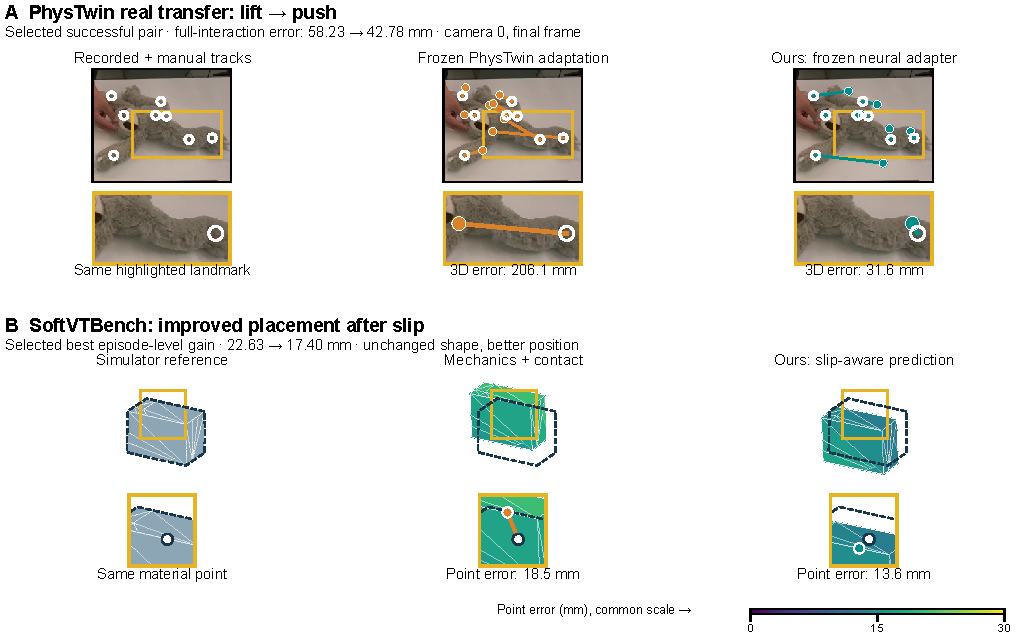
\includegraphics[width=\textwidth]{figures/public-dataset-wins.pdf}
\caption{\textbf{Where our predictions improve on public datasets.} Gold boxes identify identical enlarged regions. \textbf{A:} the successful real sloth lift-to-push transfer; the same recorded RGB appears in every panel, with white manual landmarks and colored predicted positions/error segments. These are geometric overlays, not predicted RGB. The final-frame zoom selects the largest 3D landmark improvement; other errors remain visible in the overview. \textbf{B:} the strongest episode-level SoftVT gain, at 75\% of the forecast interval, with a common point-error scale and reference outline. The zoom selects a point improving in both projected and 3D position. Local point errors differ from whole-sequence means in the headers. These selected successes illustrate the complete-cohort tables, not uniform superiority.}
\label{fig:publicwins}
\end{figure*}
\subsection{Real captures: continuation versus transfer}
\paragraph{Complete continuation benchmark.}
Eight PhysTwin plush sequences cover lifts, pushing and stretching. All were historically inspected. Our fixed corrected-mask recipe uses 240 nodes, 18 prefix fitting frames and at most 50 optimization iterations. A released transition-validity mask is shifted to the incoming transition, removing an older one-frame look-ahead; upstream offline tracking has not been certified causal. Table~\ref{tab:real} retains every sequence. The neural law improves the matched analytic adapter, but released PhysTwin and a position-regression control remain stronger on tracking.
\begin{table}[t]
\centering\small\setlength{\tabcolsep}{3pt}
\caption{\textbf{Real sequence continuation, all eight captures.} Track and internal pair-distance-change errors (mm). Image metrics use the same initial appearance at 72 recorded camera/time pairs.}
\label{tab:real}
\begin{tabular}{lrrrr}\toprule
Method & Track$\downarrow$ & Pair$\downarrow$ & PSNR$\uparrow$ & LPIPS$\downarrow$\\\midrule
Position ridge &29.04&18.85&--&--\\
Analytic adapter &40.54&18.66&16.04&.329\\
Ours, neural &39.01&16.96&16.13&.326\\
\textbf{Released PhysTwin} &\textbf{21.14}&\textbf{10.52}&\textbf{17.66}&\textbf{.264}\\\bottomrule
\end{tabular}
\end{table}
Appearance is transported identically and never refitted to future frames; crops come from the reference foreground with an eight-pixel margin. Native PhysTwin wins this shared-appearance comparison too. Unrecorded camera orbits are qualitative only because reference images do not exist there.




\paragraph{Frozen cross-interaction pilot.}
Five declared source--target pairs transfer the fitted material from single-lift sloth/zebra to another manipulation of the named object. Initial-only rigid registration must pass median/95th-percentile distance gates of 3\%/8\% of source diagonal. Two pairs pass: sloth lift to push, and zebra one-hand to two-hand lift. The other three remain reported diagnostics. No target motion after initialization is fitted. The native adaptation retains source object springs and builds geometric tool connections using median source attachment stiffness, mirroring our source-material/target-attachment split. Fitting budgets and constitutive families remain different.
\begin{table}[t]
\centering\small\setlength{\tabcolsep}{3pt}
\caption{\textbf{Real changed interaction, two qualifying pairs.} Full noninitial target trajectories; mean errors in mm. This is distinct from suffix continuation above.}
\label{tab:realtransfer}
\begin{tabular}{lrrr}\toprule
Method & Track$\downarrow$ & Displacement$\downarrow$ & Pair$\downarrow$\\\midrule
Source-shape persistence &79.11&70.79&17.25\\
Frozen PhysTwin adapt. &44.63&34.97&16.85\\
Analytic adapter &40.90&29.60&16.71\\
\textbf{Ours, neural} &\textbf{39.16}&\textbf{27.34}&\textbf{16.20}\\\bottomrule
\end{tabular}
\end{table}
Figure~\ref{fig:publicwins} localizes the sloth-push improvement. Mean tracking improves 12.26\% over frozen PhysTwin, but the two pairs have mixed outcomes: ours is better for sloth push and worse for zebra double lift. Internal-deformation improvement is 3.82\%, smaller than displacement improvement (21.81\%). The five-pair diagnostic table is retained without promoting geometrically incompatible pairs to the primary result. Projected 2D landmark error does not improve in aggregate (56.79 versus 56.20 pixels). This is a real-transfer pilot, not a broad claim of real-world OOD superiority.




\section{Analysis and Limitations}
The studies isolate different useful components. Controlled mechanics supports changed supports, gravity and contact; the matched analytic control shows that correct physical structure is at least as important as learning the law. SoftVT isolates a slip/release improvement with unchanged shape. Real neural-versus-analytic comparisons show a modest constitutive contribution, while complete continuation favors the established spring model. These findings motivate composition without claiming that every component improves every dataset.

\paragraph{Connecting appearance to mechanics.}
A dense hybrid retains PIDG's Gaussian appearance and temporal map while applying our frozen material decoder and inferred Gaussian load fields to its shared deformation field. On Balls Reaction, Rubber Duck and Motion Kuro, held-image PSNR is 49.51/49.54, 41.59/41.82, 39.79/39.92\,dB (hybrid/native; 138 images, $320\times180$). 3 of three scenes meet the predeclared rendering-parity tolerance. This resolves the coarse adapter's large appearance penalty, but the soft constraint does not establish new-action prediction or force identification. The supplement reports all candidates, resolutions and the earlier equilibrium diagnostic.

\paragraph{Scope and reproducibility.}
The primary physical-response studies supply geometry and correspondences; some supply density and boundary laws. The supplementary dense PIDG hybrid uses reconstruction-derived neighborhoods and soft mechanical constraints. Initial-state uncertainty, image tracking, unmodeled dissipation and discretization can dominate material inference. The coupled simulator and reduced benchmark adapters support different contact assumptions. We report physical diagnostics and reference sensitivity rather than presenting them as a universal realism certificate. Exact protocols, source hashes, fitting budgets, per-case tables and figure selection accompany the manuscript. No predictions are tuned or selected by their future error for this consolidation.

\section{Conclusion}
Separating material response from tool and environmental interactions yields useful position-driven twins across controlled contact scenes and two external datasets. The gains concern specific physical responses, not uniform superiority: analytic mechanics is competitive, native PhysTwin wins ordinary real continuation, and uncertainty remains poorly calibrated. Evaluating changed responses, internal deformation and rendering separately gives a more informative test of a digital twin than visual agreement alone.
\clearpage
\section*{LLM Usage Statement}
OpenAI Codex assisted with implementation, experiment orchestration, literature discovery, evidence audits, manuscript drafting and programmatic figure generation. Results come from saved experiment artifacts; scientific figures are generated from those artifacts rather than synthesized as evidence. Authors remain responsible for validating methods, results, references and the final submission.
{\small\bibliographystyle{ieeenat_fullname}\bibliography{references}}
\end{document}
